\documentclass[12pt]{article}
\usepackage{verbatim}
\usepackage[dvips]{epsfig}
\usepackage{color}
\usepackage{url}
\usepackage[colorlinks=true]{hyperref}

\begin{document}

\section*{GENESIS: Documentation}

{\bf Related Documentation:}
% start: userdocs-tag-replace-items related-do-nothing
% end: userdocs-tag-replace-items related-do-nothing

\section*{De Schutter: Purkinje Cell Model}

\begin{figure}[h]
\centering
   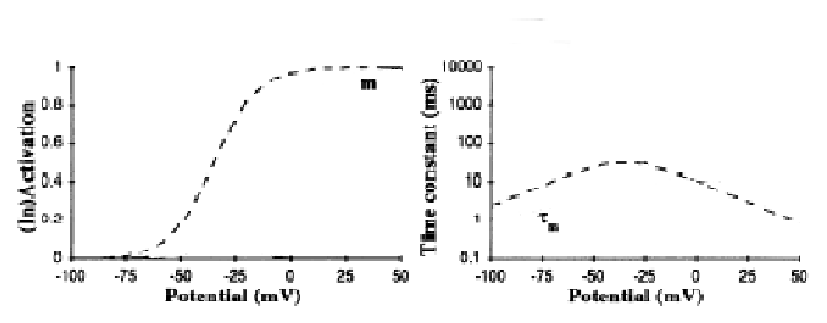
\includegraphics[scale=0.75]{figures/DS1.2E2.eps}
   \caption{Activation properties of the persistent K$^+$ current (Km, - - -, no inactivation) in the model. Seady-state activation vs. voltage is plotted at the {\em left} and the time constant of activation ($\tau_m$) vs. voltage on the {\em right} (Note: Semilogarithmic scale). The Km current does not inactivate.}
   \label{fig:DS1.2E2}
\end{figure}

\subsection*{Persistent Potassium Current (Km)}

Noninactivating K$^+$ channels in Purkinje cells have been reported by\,\cite{Bossu:1989kl} and are also apparent in recordings from\,\cite{Hirano:1989uq}. No kinetic data were available from Purkinje cells, so we have again used the equations of\,\cite{Yamada-W:1989bs} for the noninactivating muscarinic K$^+$ channel (Km).

\bibliographystyle{plain}
\bibliography{../tex/bib/g3-refs}

\end{document}
